\begin{figure}
  \centering
  \begin{tabular}{c}
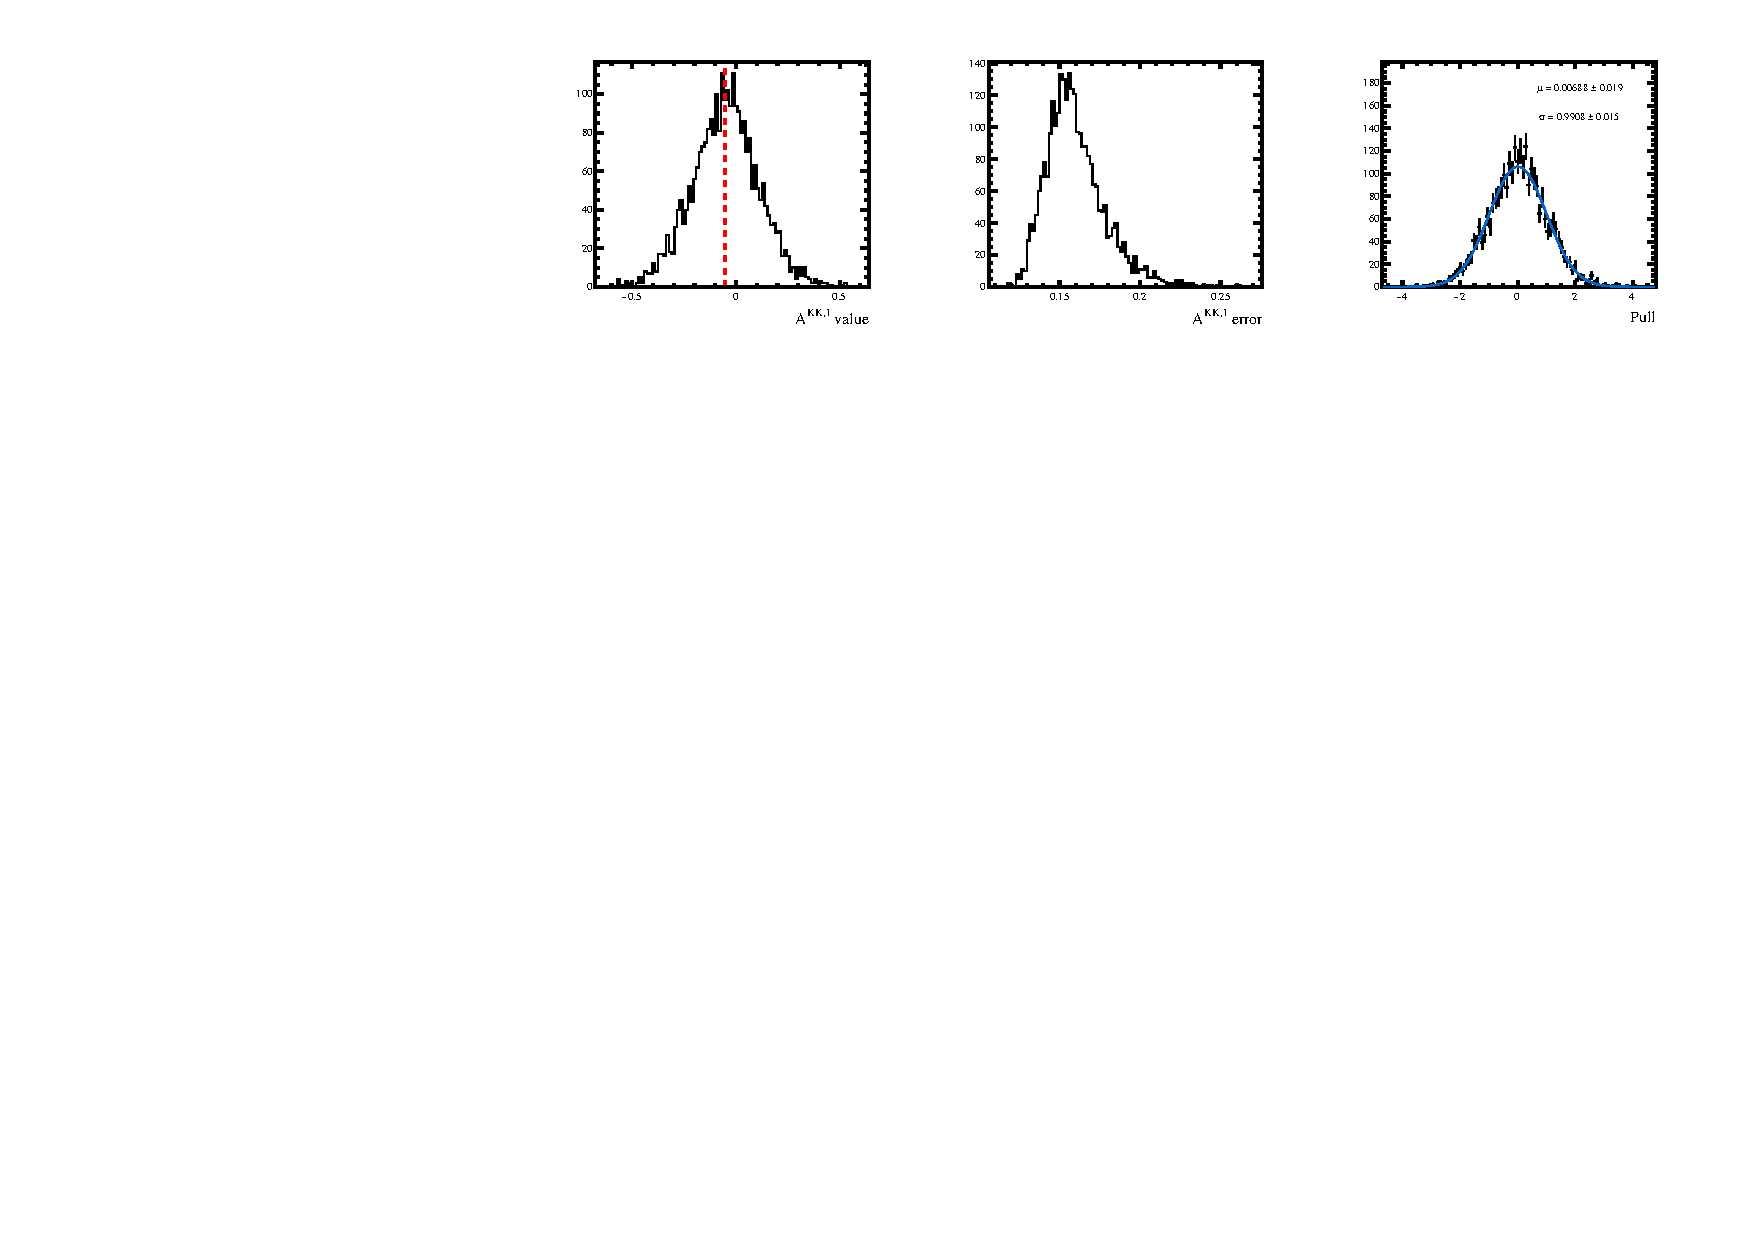
\includegraphics[width=0.7\textwidth]{ANA_resources/Plots/Data_fit/FitterBias//A_signal_KK_run1.pdf} \\
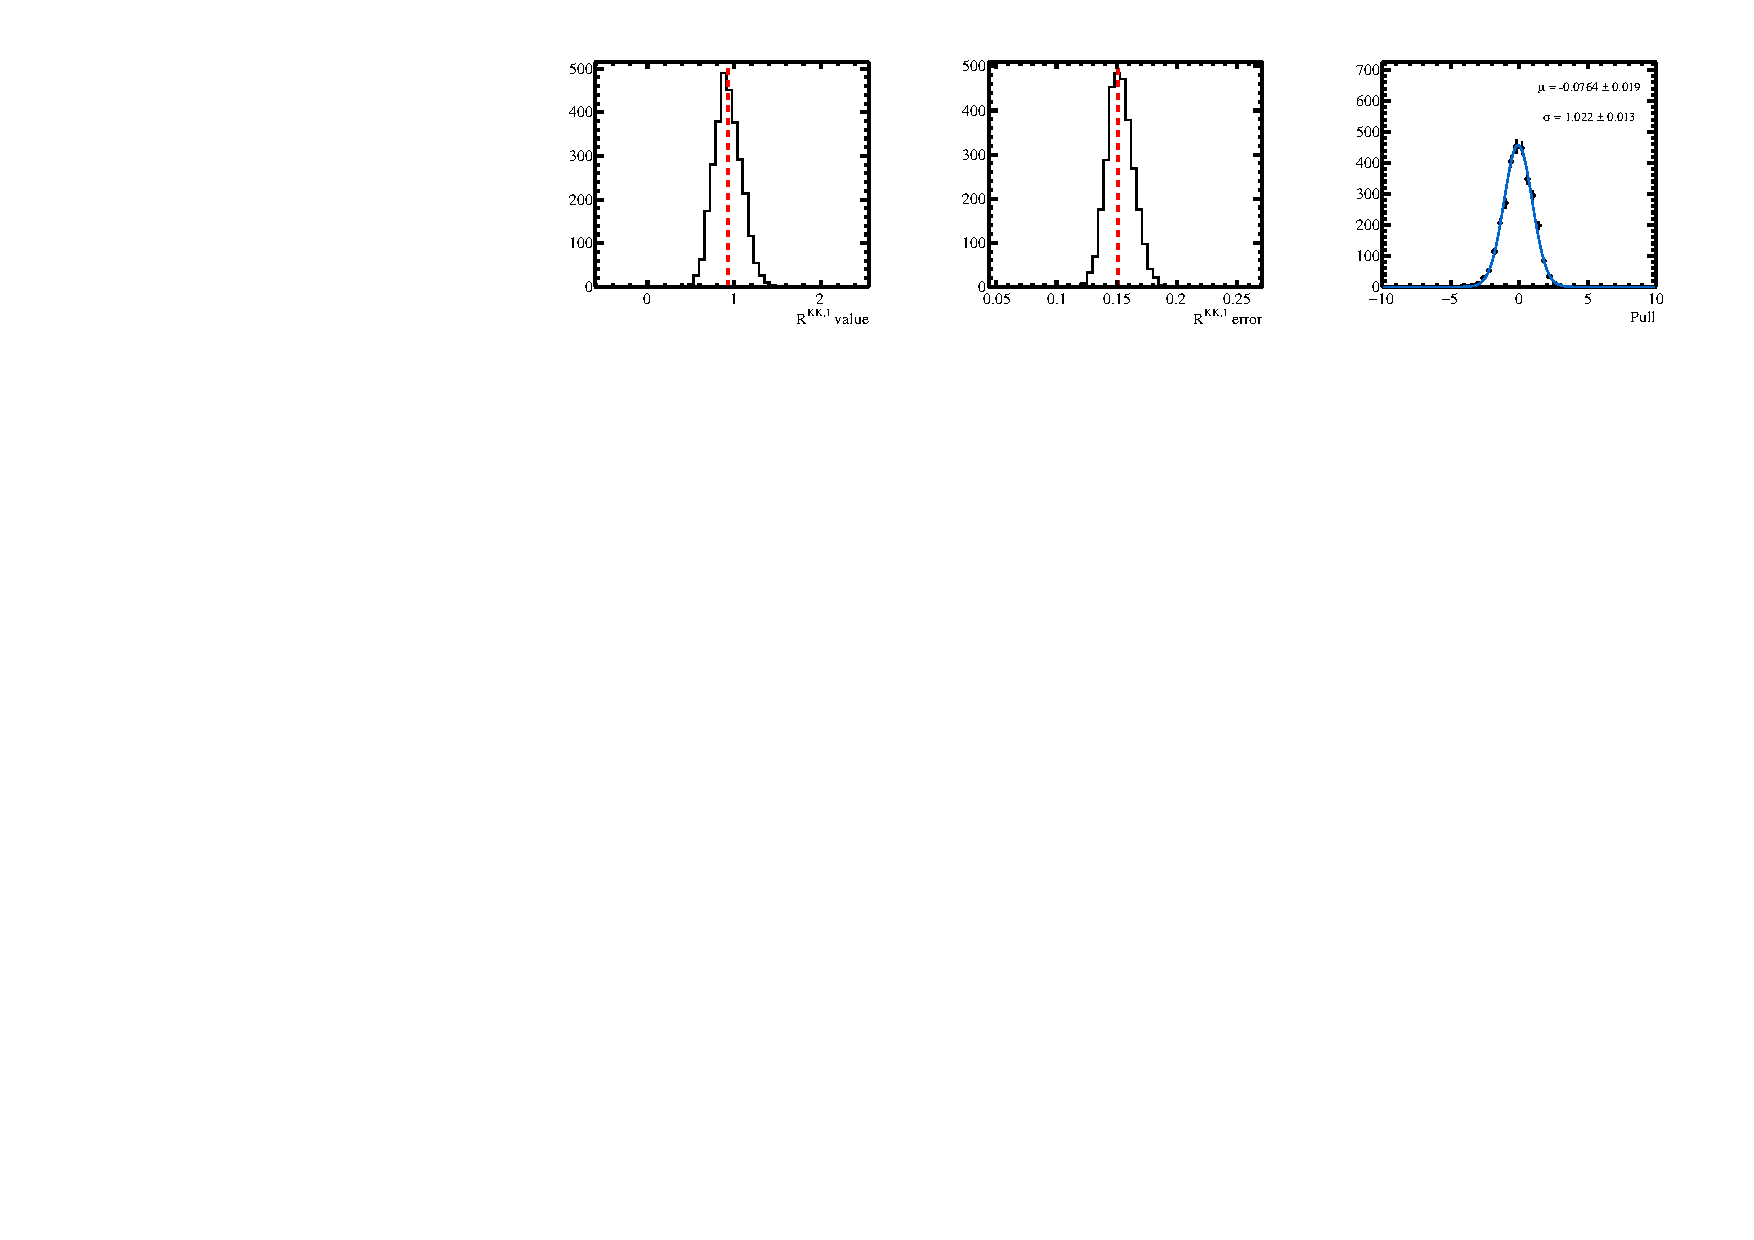
\includegraphics[width=0.7\textwidth]{ANA_resources/Plots/Data_fit/FitterBias//R_signal_KK_run1.pdf} \\
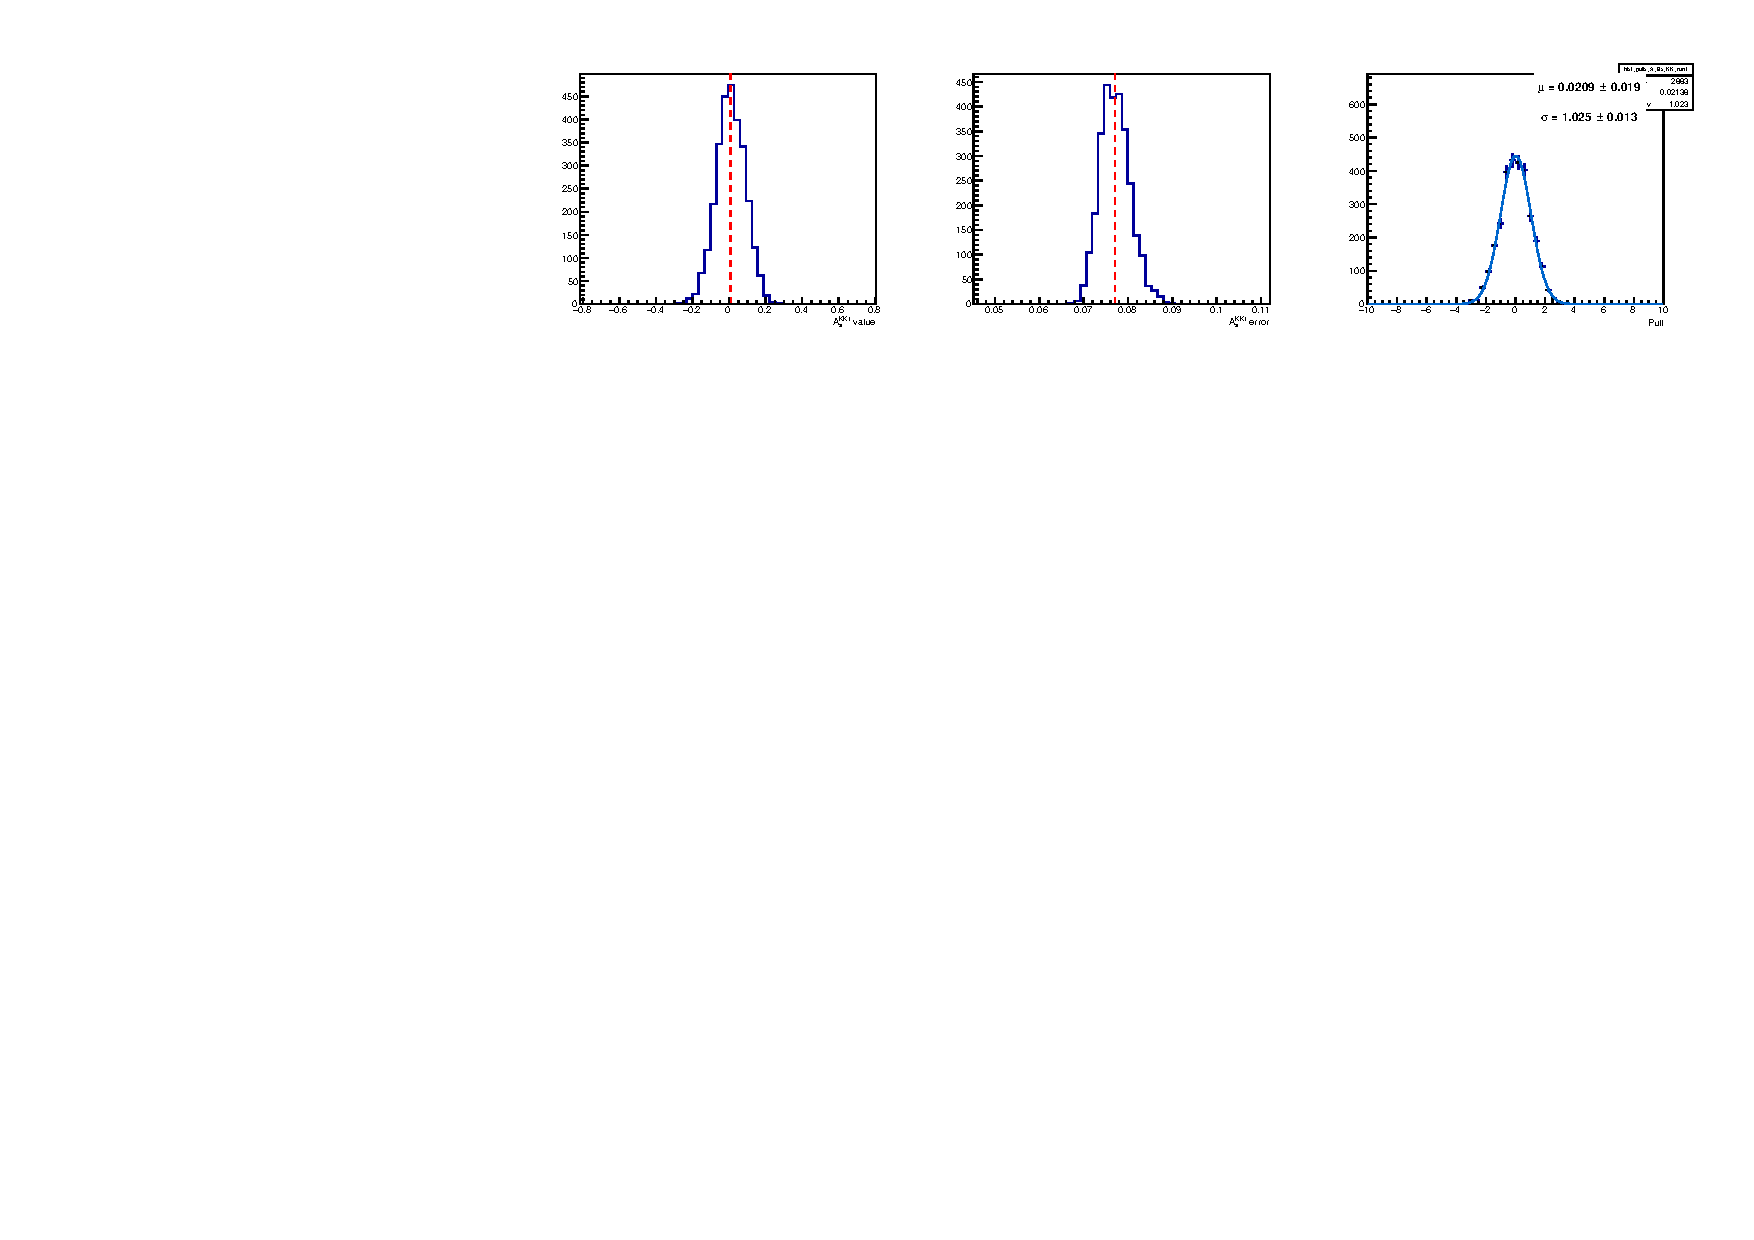
\includegraphics[width=0.7\textwidth]{ANA_resources/Plots/Data_fit/FitterBias//A_Bs_KK_run1.pdf} \\
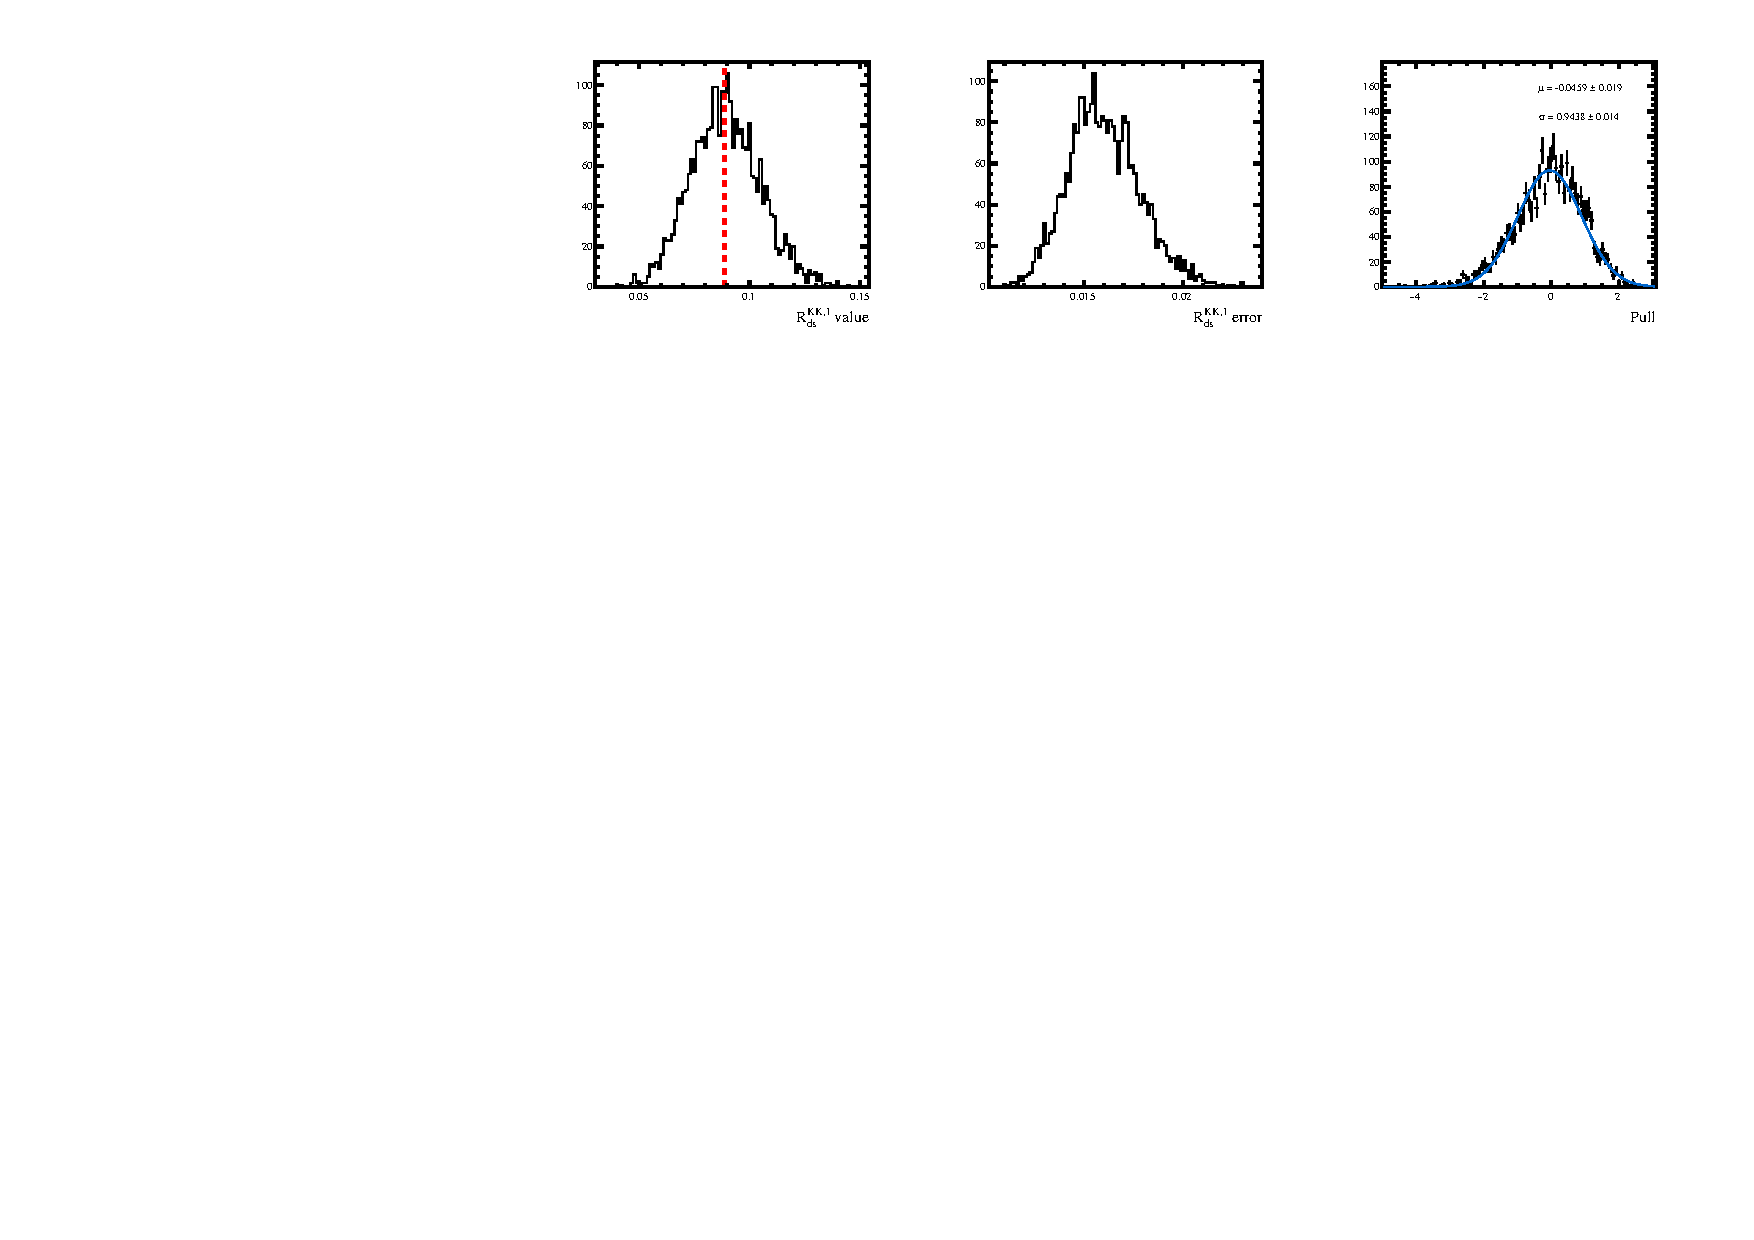
\includegraphics[width=0.7\textwidth]{ANA_resources/Plots/Data_fit/FitterBias//R_ds_KK_run1.pdf} \\
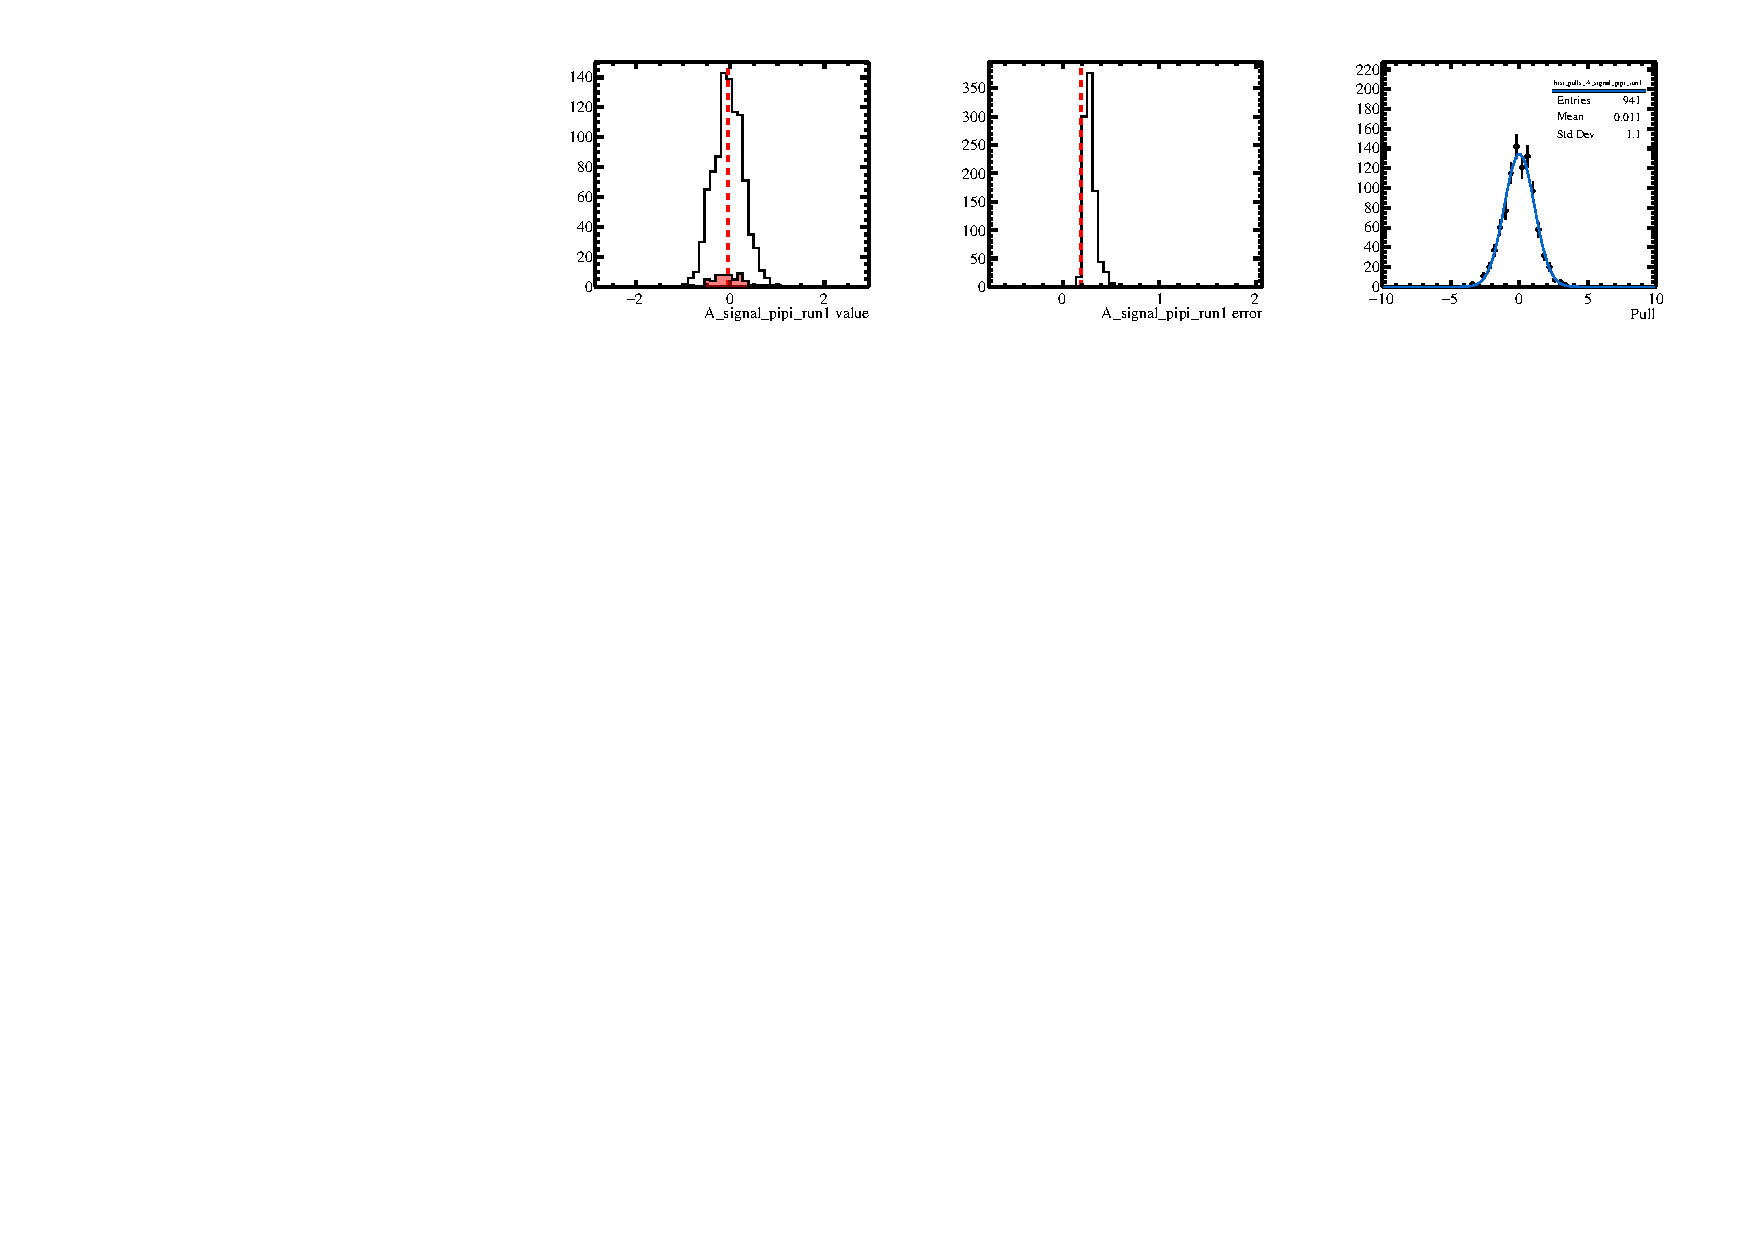
\includegraphics[width=0.7\textwidth]{ANA_resources/Plots/Data_fit/FitterBias//A_signal_pipi_run1.pdf} \\
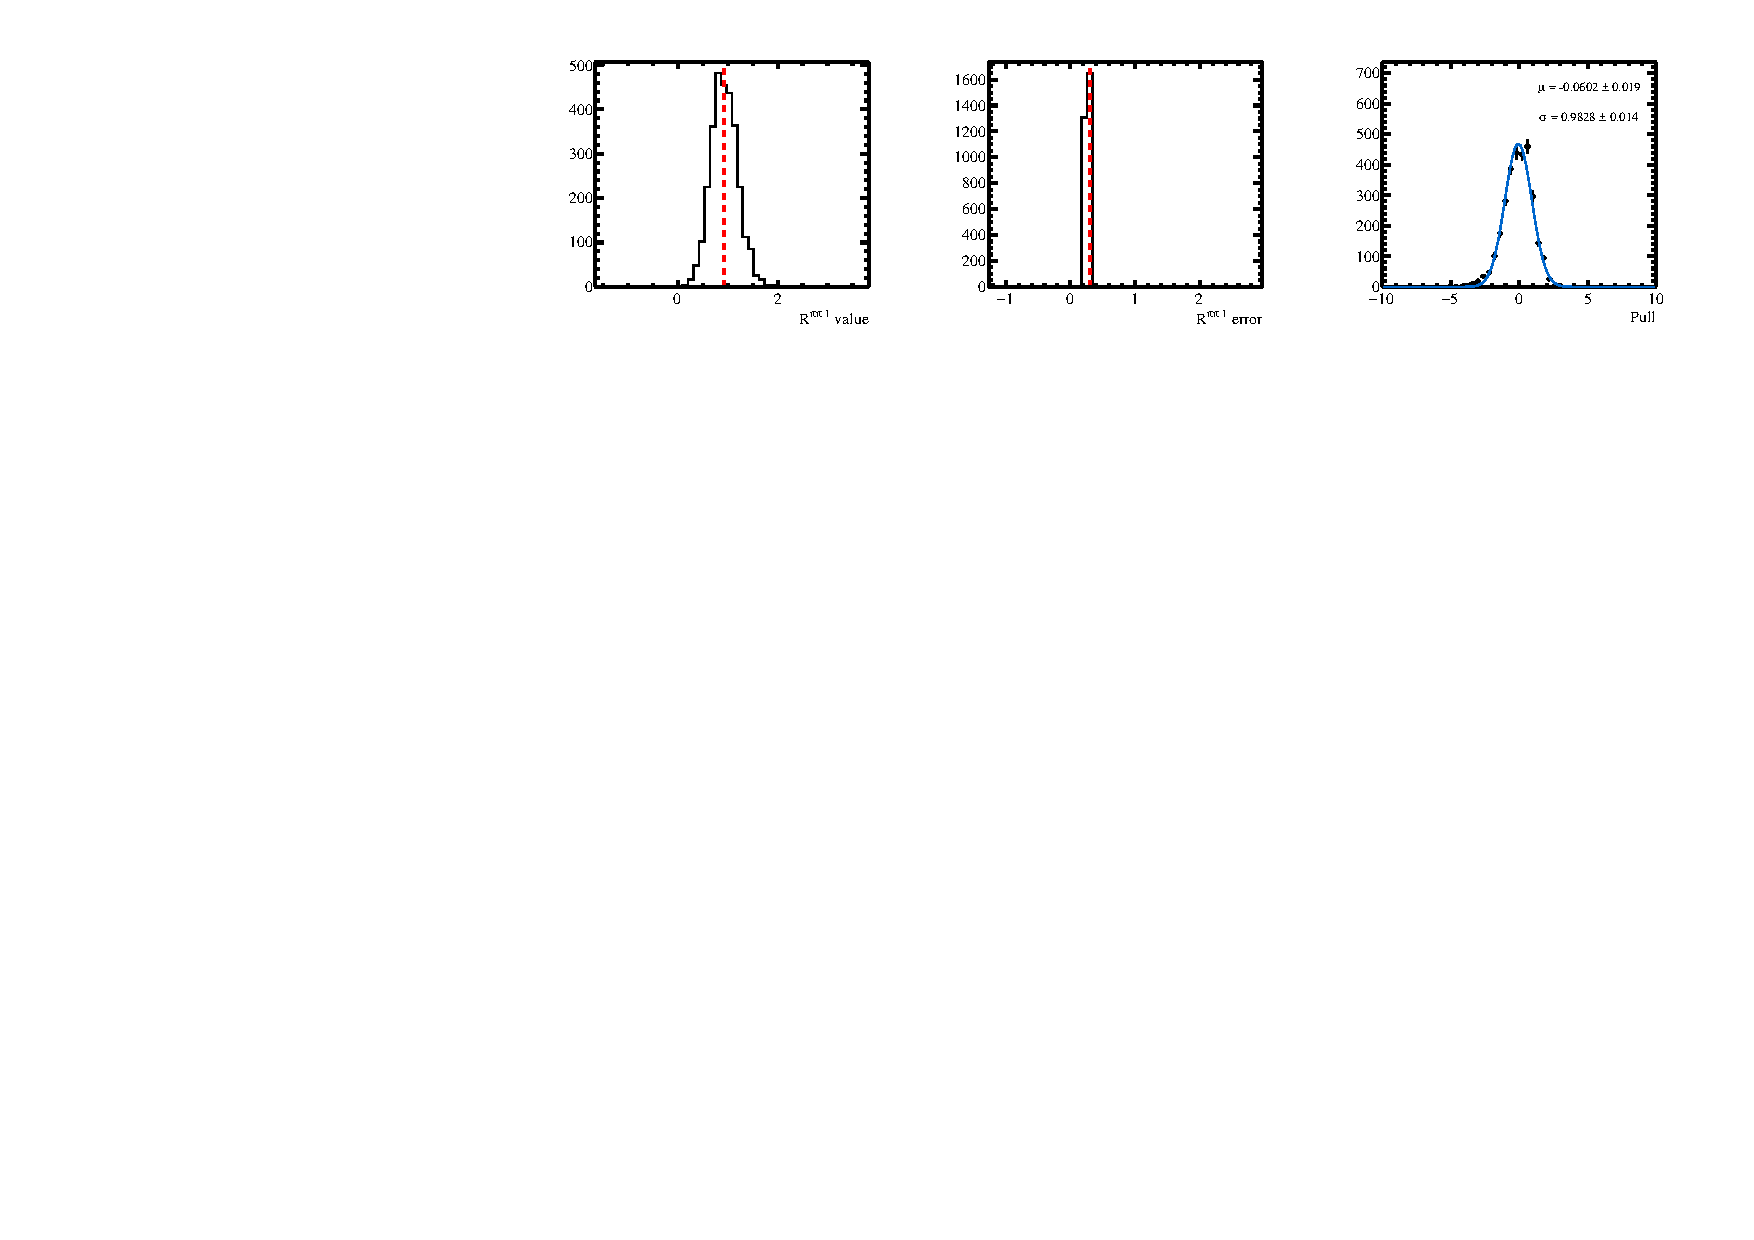
\includegraphics[width=0.7\textwidth]{ANA_resources/Plots/Data_fit/FitterBias//R_signal_pipi_run1.pdf} \\
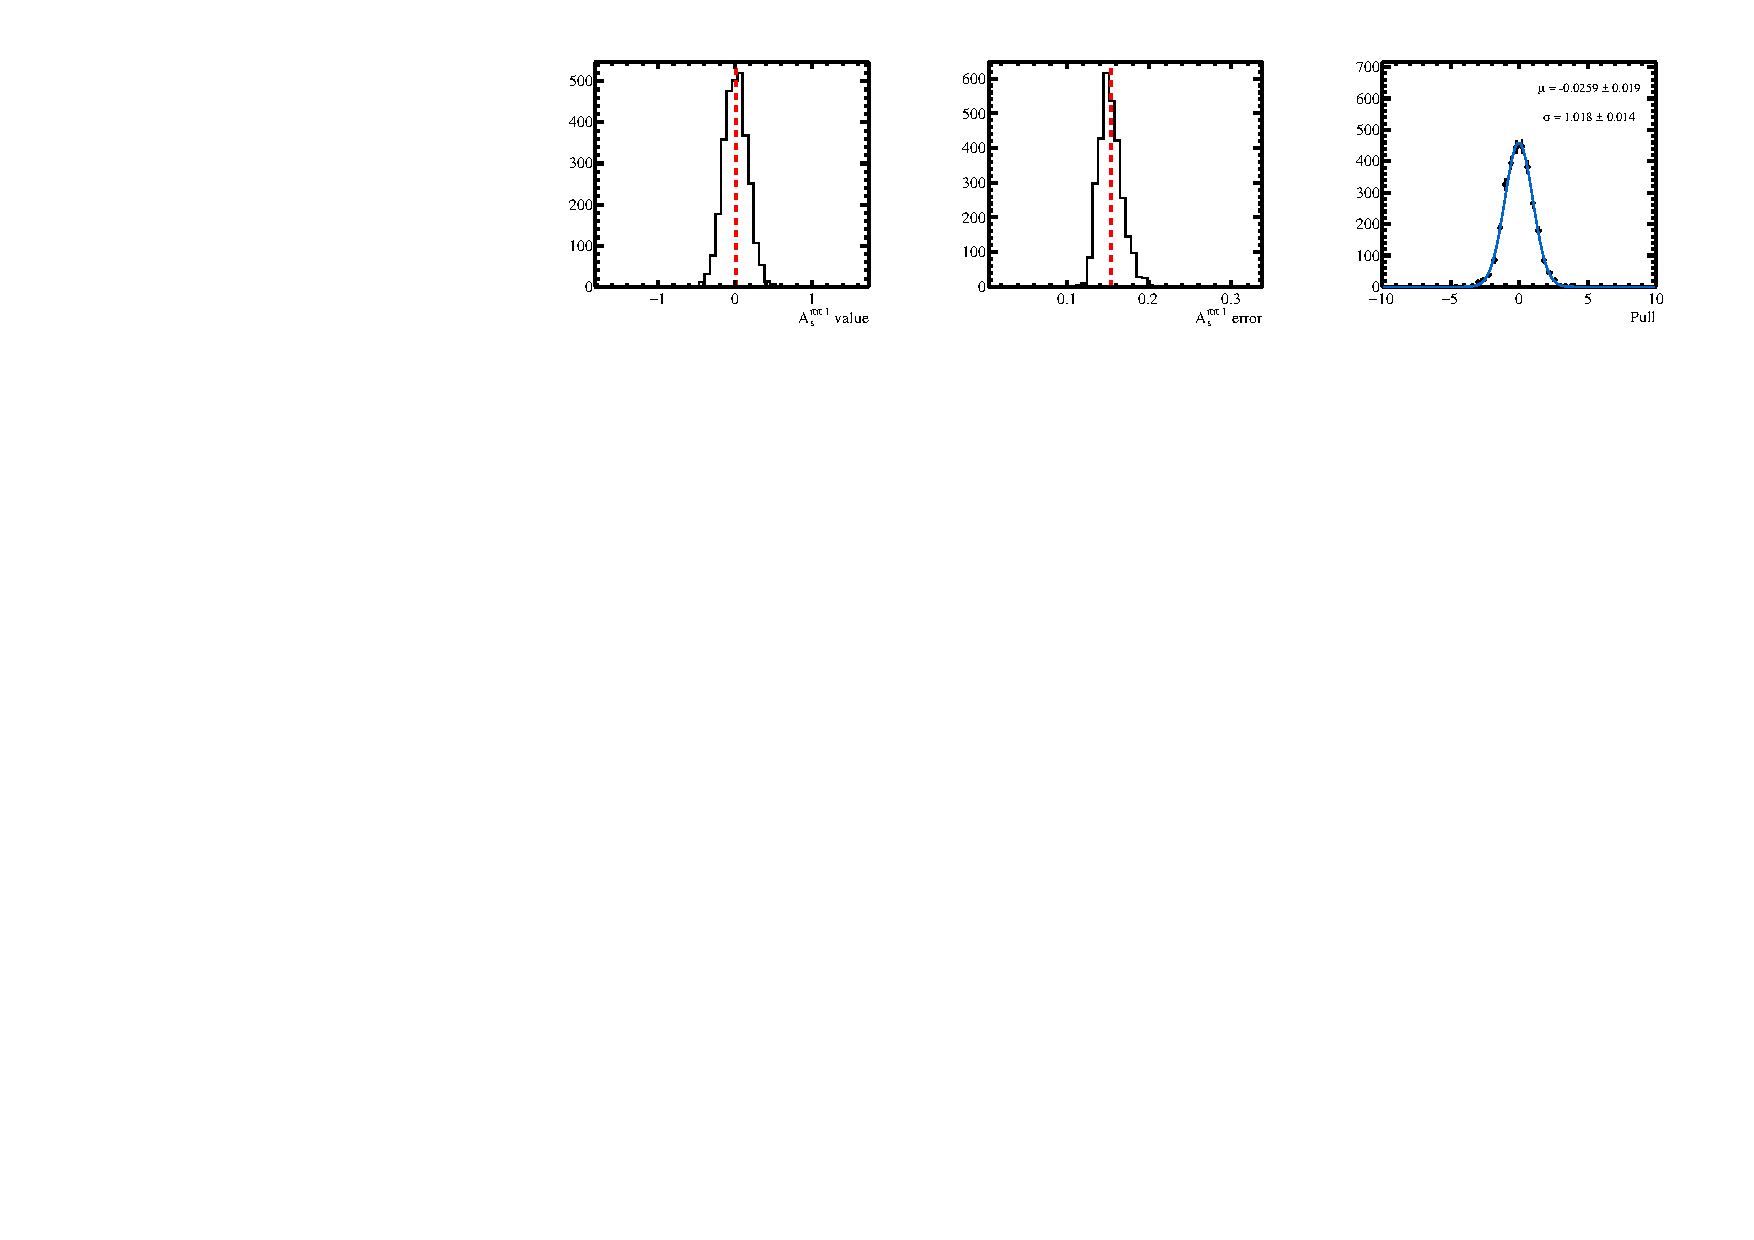
\includegraphics[width=0.7\textwidth]{ANA_resources/Plots/Data_fit/FitterBias//A_Bs_pipi_run1.pdf} \\
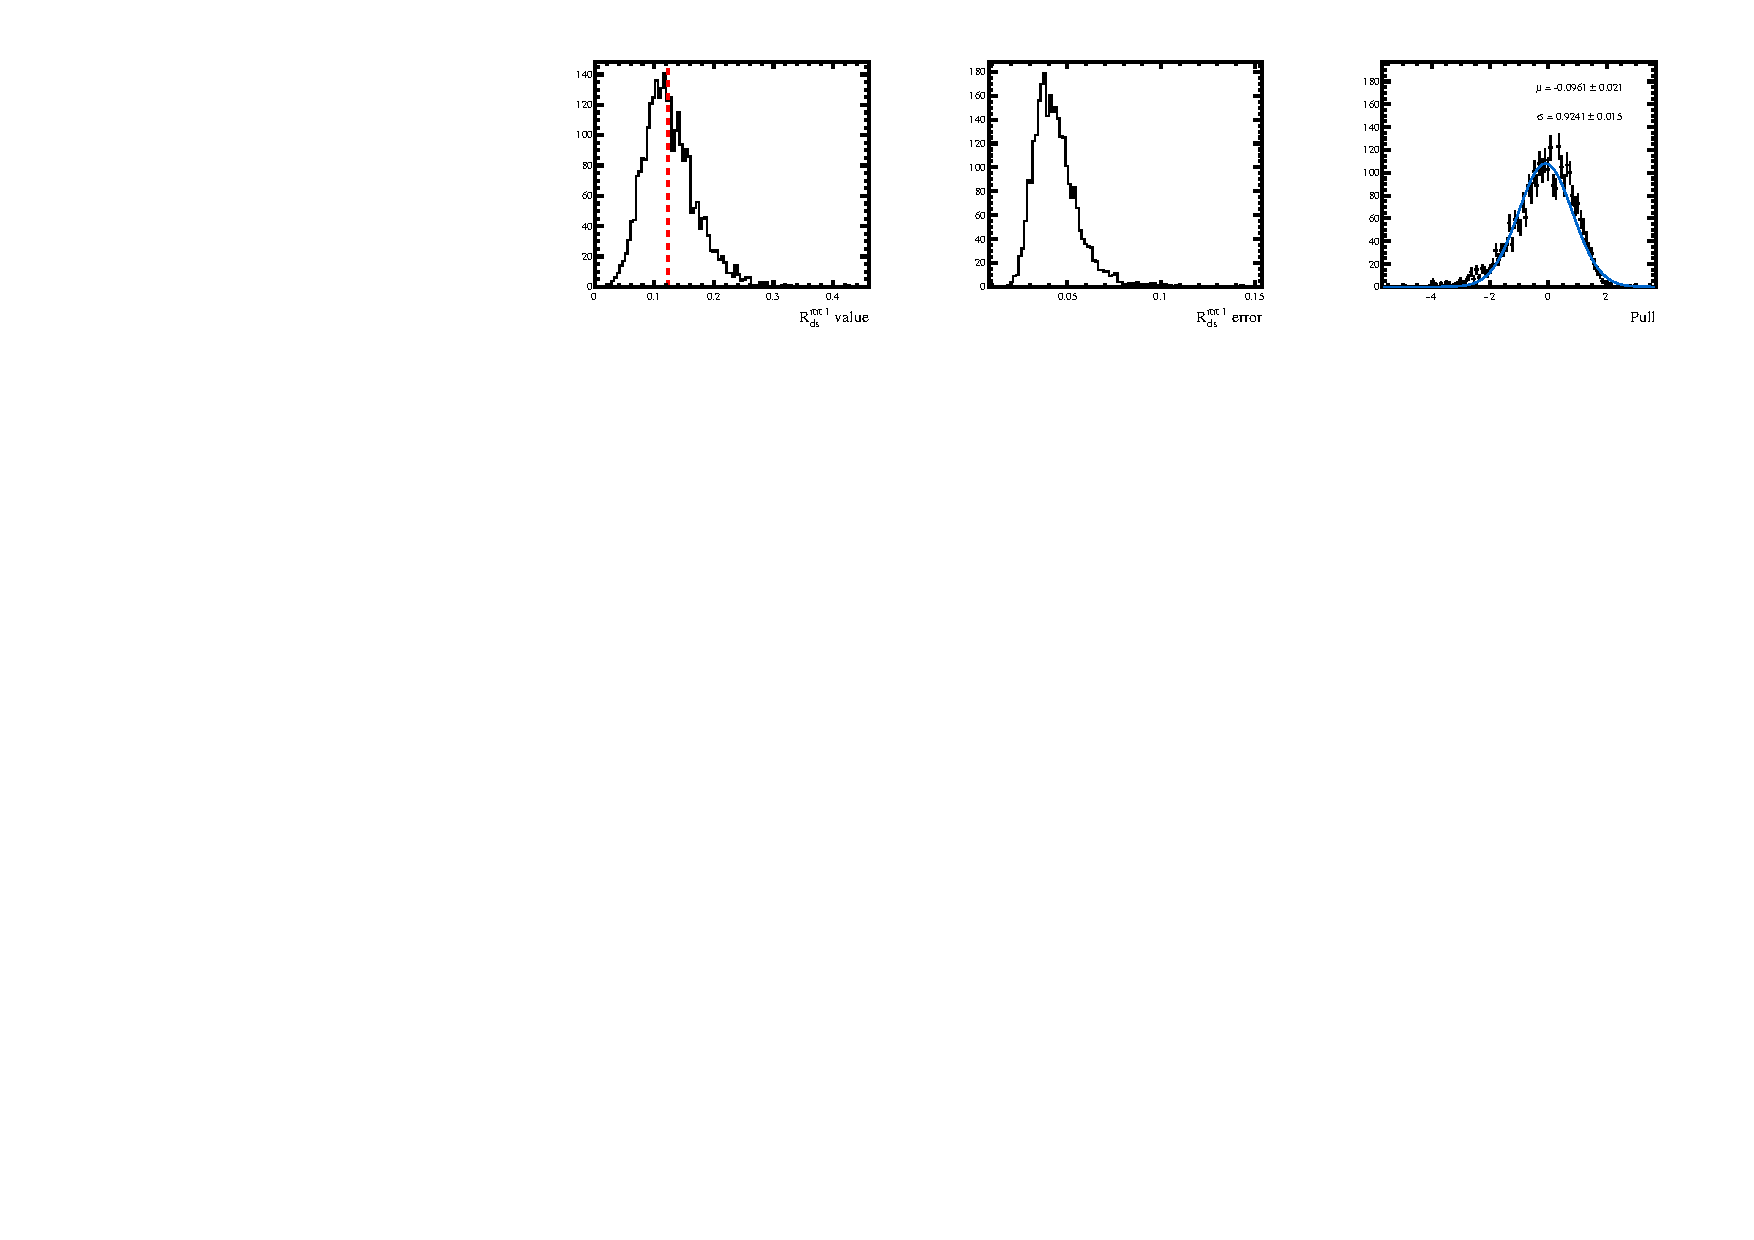
\includegraphics[width=0.7\textwidth]{ANA_resources/Plots/Data_fit/FitterBias//R_ds_pipi_run1.pdf} \\
  \end{tabular}
  \caption{Pull plots for Run 1 GLW parameters of interest, obtained from generating and fitting 1000 toys using the data fit model.}
\label{fig:GLW_run1_pulls}
\end{figure}
